\chapter{Dictionaries}

\index{dictionary}
\index{dictionary}
\index{type!dict}
\index{key}
\index{key-value pair}
\index{index}
A {\bf dictionary} is like a list, but more general.  In a list,
the indices have to be integers; in a dictionary they can
be (almost) any type.

You can think of a dictionary as a mapping between a set of indices
(which are called {\bf keys}) and a set of values.  Each key maps to a
value.  The association of a key and a value is called a {\bf
  key-value pair} or sometimes an {\bf item}.

As an example, we'll build a dictionary that maps from English
to Spanish words, so the keys and the values are all strings.

The function {\tt dict} creates a new dictionary with no items.
Because {\tt dict} is the name of a built-in function, you
should avoid using it as a variable name.
\index{dict function}
\index{function!dict}

\begin{verbatim}
>>> eng2sp = dict()
>>> print eng2sp
{}
\end{verbatim}

The squiggly-brackets, \verb"{}", represent an empty dictionary.
To add items to the dictionary, you can use square brackets:
\index{squiggly bracket}
\index{bracket!squiggly}

\begin{verbatim}
>>> eng2sp['one'] = 'uno'
\end{verbatim}
%
This line creates an item that maps from the key
{\tt 'one'} to the value \verb"'uno'".  If we print the
dictionary again, we see a key-value pair with a colon
between the key and value:

\begin{verbatim}
>>> print eng2sp
{'one': 'uno'}
\end{verbatim}
%
This output format is also an input format.  For example,
you can create a new dictionary with three items:

\begin{verbatim}
>>> eng2sp = {'one': 'uno', 'two': 'dos', 'three': 'tres'}
\end{verbatim}
%
But if you print {\tt eng2sp}, you might be surprised:

\begin{verbatim}
>>> print eng2sp
{'one': 'uno', 'three': 'tres', 'two': 'dos'}
\end{verbatim}
%
The order of the key-value pairs is not the same.  In fact, if
you type the same example on your computer, you might get a
different result.  In general, the order of items in
a dictionary is unpredictable.

But that's not a problem because
the elements of a dictionary are never indexed with integer indices.
Instead, you use the keys to look up the corresponding values:

\begin{verbatim}
>>> print eng2sp['two']
'dos'
\end{verbatim}
%
The key {\tt 'two'} always maps to the value \verb"'dos'" so the order
of the items doesn't matter.

If the key isn't in the dictionary, you get an exception:
\index{exception!KeyError}
\index{KeyError}

\begin{verbatim}
>>> print eng2sp['four']
KeyError: 'four'
\end{verbatim}
%
The {\tt len} function works on dictionaries; it returns the
number of key-value pairs:
\index{len function}
\index{function!len}

\begin{verbatim}
>>> len(eng2sp)
3
\end{verbatim}
%
The {\tt in} operator works on dictionaries; it tells you whether
something appears as a {\em key} in the dictionary (appearing
as a value is not good enough).
\index{membership!dictionary}
\index{in operator}
\index{operator!in}

\begin{verbatim}
>>> 'one' in eng2sp
True
>>> 'uno' in eng2sp
False
\end{verbatim}
%
To see whether something appears as a value in a dictionary, you
can use the method {\tt values}, which returns the values as
a list, and then use the {\tt in} operator:
\index{values method}
\index{method!values}

\begin{verbatim}
>>> vals = eng2sp.values()
>>> 'uno' in vals
True
\end{verbatim}
%
The {\tt in} operator uses different algorithms for lists and
dictionaries.  For lists, it uses a search algorithm, as in
Section~\ref{find}.  As the list gets longer, the search time gets
longer in direct proportion.  For dictionaries, Python uses an
algorithm called a {\bf hashtable} that has a remarkable property: the
{\tt in} operator takes about the same amount of time no matter how
many items there are in a dictionary.  I won't explain how that's
possible, but you can read more about it at
\url{http://en.wikipedia.org/wiki/Hash_table}.
\index{hashtable}

\begin{exercise}
\label{wordlist2}
\index{set membership}
\index{membership!set}

Write a function that reads the words in {\tt words.txt} and
stores them as keys in a dictionary.  It doesn't matter what the
values are.  Then you can use the {\tt in} operator
as a fast way to check whether a string is in
the dictionary.

If you did Exercise~\ref{wordlist1}, you can compare the speed
of this implementation with the list {\tt in} operator and the
bisection search.

\end{exercise}


\section{Dictionary as a set of counters}
\label{histogram}
\index{counter}

Suppose you are given a string and you want to count how many
times each letter appears.  There are several ways you could do it:

\begin{enumerate}

\item You could create 26 variables, one for each letter of the
alphabet.  Then you could traverse the string and, for each
character, increment the corresponding counter, probably using
a chained conditional.

\item You could create a list with 26 elements.  Then you could
convert each character to a number (using the built-in function
{\tt ord}), use the number as an index into the list, and increment
the appropriate counter.

\item You could create a dictionary with characters as keys
and counters as the corresponding values.  The first time you
see a character, you would add an item to the dictionary.  After
that you would increment the value of an existing item.

\end{enumerate}

Each of these options performs the same computation, but each
of them implements that computation in a different way.
\index{implementation}

An {\bf implementation} is a way of performing a computation;
some implementations are better than others.  For example,
an advantage of the dictionary implementation is that we don't
have to know ahead of time which letters appear in the string
and we only have to make room for the letters that do appear.

Here is what the code might look like:

\begin{verbatim}
def histogram(s):
    d = dict()
    for c in s:
        if c not in d:
            d[c] = 1
        else:
            d[c] += 1
    return d
\end{verbatim}
%
The name of the function is {\bf histogram}, which is a statistical
term for a set of counters (or frequencies).
\index{histogram}
\index{frequency}
\index{traversal}

The first line of the
function creates an empty dictionary.  The {\tt for} loop traverses
the string.  Each time through the loop, if the character {\tt c} is
not in the dictionary, we create a new item with key {\tt c} and the
initial value 1 (since we have seen this letter once).  If {\tt c} is
already in the dictionary we increment {\tt d[c]}.
\index{histogram}

Here's how it works:

\begin{verbatim}
>>> h = histogram('brontosaurus')
>>> print h
{'a': 1, 'b': 1, 'o': 2, 'n': 1, 's': 2, 'r': 2, 'u': 2, 't': 1}
\end{verbatim}
%
The histogram indicates that the letters {\tt 'a'} and \verb"'b'"
appear once; \verb"'o'" appears twice, and so on.

\begin{exercise}
\index{get method}
\index{method!get}

Dictionaries have a method called {\tt get} that takes a key
and a default value.  If the key appears in the dictionary,
{\tt get} returns the corresponding value; otherwise it returns
the default value.  For example:

\begin{verbatim}
>>> h = histogram('a')
>>> print h
{'a': 1}
>>> h.get('a', 0)
1
>>> h.get('b', 0)
0
\end{verbatim}
%
Use {\tt get} to write {\tt histogram} more concisely.  You
should be able to eliminate the {\tt if} statement.
\end{exercise}


\section{Looping and dictionaries}
\index{dictionary!looping with}
\index{looping!with dictionaries}
\index{traversal}

If you use a dictionary in a {\tt for} statement, it traverses
the keys of the dictionary.  For example, \verb"print_hist"
prints each key and the corresponding value:

\begin{verbatim}
def print_hist(h):
    for c in h:
        print c, h[c]
\end{verbatim}
%
Here's what the output looks like:

\begin{verbatim}
>>> h = histogram('parrot')
>>> print_hist(h)
a 1
p 1
r 2
t 1
o 1
\end{verbatim}
%
Again, the keys are in no particular order.

\begin{exercise}
\index{keys method}
\index{method!keys}

Dictionaries have a method called {\tt keys} that returns
the keys of the dictionary, in no particular order, as a list.

Modify \verb"print_hist" to print the keys and their values
in alphabetical order.
\end{exercise}



\section{Reverse lookup}
\label{raise}
\index{dictionary!lookup}
\index{dictionary!reverse lookup}
\index{lookup, dictionary}
\index{reverse lookup, dictionary}

Given a dictionary {\tt d} and a key {\tt k}, it is easy to
find the corresponding value {\tt v = d[k]}.  This operation
is called a {\bf lookup}.

But what if you have {\tt v} and you want to find {\tt k}?
You have two problems: first, there might be more than one
key that maps to the value {\tt v}.  Depending on the application,
you might be able to pick one, or you might have to make
a list that contains all of them.  Second, there is no
simple syntax to do a {\bf reverse lookup}; you have to search.

Here is a function that takes a value and returns the first
key that maps to that value:

\begin{verbatim}
def reverse_lookup(d, v):
    for k in d:
        if d[k] == v:
            return k
    raise ValueError
\end{verbatim}
%
This function is yet another example of the search pattern, but it
uses a feature we haven't seen before, {\tt raise}.  The {\tt raise}
statement causes an exception; in this case it causes a {\tt
  ValueError}, which generally indicates that there is something wrong
with the value of a parameter.
\index{search}
\index{pattern!search}
\index{raise statement}
\index{statement!raise}
\index{exception!ValueError}
\index{ValueError}

If we get to the end of the loop, that means {\tt v}
doesn't appear in the dictionary as a value, so we raise an
exception.

Here is an example of a successful reverse lookup:

\begin{verbatim}
>>> h = histogram('parrot')
>>> k = reverse_lookup(h, 2)
>>> print k
r
\end{verbatim}
%
And an unsuccessful one:

\begin{verbatim}
>>> k = reverse_lookup(h, 3)
Traceback (most recent call last):
  File "<stdin>", line 1, in ?
  File "<stdin>", line 5, in reverse_lookup
ValueError
\end{verbatim}
%
The result when you raise an exception is the same as when
Python raises one: it prints a traceback and an error message.
\index{traceback}
\index{optional argument}
\index{argument!optional}

The {\tt raise} statement takes a detailed error message as an
optional argument.  For example:

\begin{verbatim}
>>> raise ValueError('value does not appear in the dictionary')
Traceback (most recent call last):
  File "<stdin>", line 1, in ?
ValueError: value does not appear in the dictionary
\end{verbatim}
%
A reverse lookup is much slower than a forward lookup; if you
have to do it often, or if the dictionary gets big, the performance
of your program will suffer.

\begin{exercise}

Modify \verb"reverse_lookup" so that it builds and returns a list
of {\em all} keys that map to {\tt v}, or an empty list if there
are none.

\end{exercise}


\section{Dictionaries and lists}
\label{invert}

Lists can appear as values in a dictionary.  For example, if you
were given a dictionary that maps from letters to frequencies, you
might want to invert it; that is, create a dictionary that maps
from frequencies to letters.  Since there might be several letters
with the same frequency, each value in the inverted dictionary
should be a list of letters.
\index{invert dictionary}
\index{dictionary!invert}

Here is a function that inverts a dictionary:

\begin{verbatim}
def invert_dict(d):
    inverse = dict()
    for key in d:
        val = d[key]
        if val not in inverse:
            inverse[val] = [key]
        else:
            inverse[val].append(key)
    return inverse
\end{verbatim}
%
Each time through the loop, {\tt key} gets a key from {\tt d} and 
{\tt val} gets the corresponding value.  If {\tt val} is not in {\tt inverse},
that means we haven't seen it before, so we create a new item and
initialize it with a {\bf singleton} (a list that contains a
single element).  Otherwise we have seen this value before, so we
append the corresponding key to the list.
\index{singleton}

Here is an example:

\begin{verbatim}
>>> hist = histogram('parrot')
>>> print hist
{'a': 1, 'p': 1, 'r': 2, 't': 1, 'o': 1}
>>> inverse = invert_dict(hist)
>>> print inverse
{1: ['a', 'p', 't', 'o'], 2: ['r']}
\end{verbatim}

\begin{figure}
\centerline
{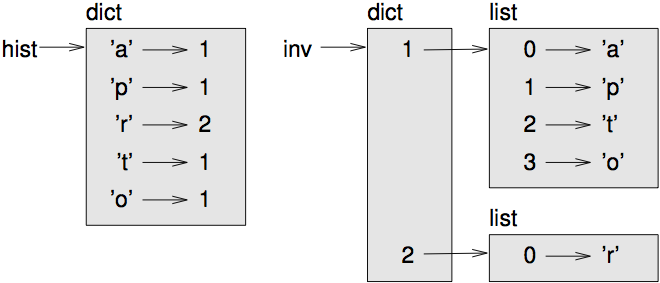
\includegraphics[scale=0.8]{figs/dict1.pdf}}
\caption{State diagram.}
\label{fig.dict1}
\end{figure}

Figure~\ref{fig.dict1} is a state diagram showing {\tt hist} and {\tt inverse}.
A dictionary is represented as a box with the type {\tt dict} above it
and the key-value pairs inside.  If the values are integers, floats or
strings, I usually draw them inside the box, but I usually draw lists
outside the box, just to keep the diagram simple.
\index{state diagram}
\index{diagram!state}

Lists can be values in a dictionary, as this example shows, but they
cannot be keys.  Here's what happens if you try:
\index{TypeError}
\index{exception!TypeError}


\begin{verbatim}
>>> t = [1, 2, 3]
>>> d = dict()
>>> d[t] = 'oops'
Traceback (most recent call last):
  File "<stdin>", line 1, in ?
TypeError: list objects are unhashable
\end{verbatim}
%
I mentioned earlier that a dictionary is implemented using
a hashtable and that means that the keys have to be {\bf hashable}.
\index{hash function}
\index{hashable}

A {\bf hash} is a function that takes a value (of any kind)
and returns an integer.  Dictionaries use these integers,
called hash values, to store and look up key-value pairs.
\index{immutability}

This system works fine if the keys are immutable.  But if the
keys are mutable, like lists, bad things happen.  For example,
when you create a key-value pair, Python hashes the key and 
stores it in the corresponding location.  If you modify the
key and then hash it again, it would go to a different location.
In that case you might have two entries for the same key,
or you might not be able to find a key.  Either way, the
dictionary wouldn't work correctly.

That's why the keys have to be hashable, and why mutable types like
lists aren't.  The simplest way to get around this limitation is to
use tuples, which we will see in the next chapter.

Since lists and dictionaries are mutable, they can't be used as keys,
but they {\em can} be used as values.

\begin{exercise}
Read the documentation of the dictionary method {\tt setdefault}
and use it to write a more concise version of \verb"invert_dict".
Solution: \url{http://thinkpython.com/code/invert_dict.py}.
\index{setdefault method}
\index{method!setdefault}

\end{exercise}


\section{Memos}

If you played with the {\tt fibonacci} function from
Section~\ref{one.more.example}, you might have noticed that the bigger
the argument you provide, the longer the function takes to run.
Furthermore, the run time increases very quickly.
\index{fibonacci function}
\index{function!fibonacci}

To understand why, consider Figure~\ref{fig.fibonacci}, which shows
the {\bf call graph} for {\tt fibonacci} with {\tt n=4}:

\begin{figure}
\centerline
{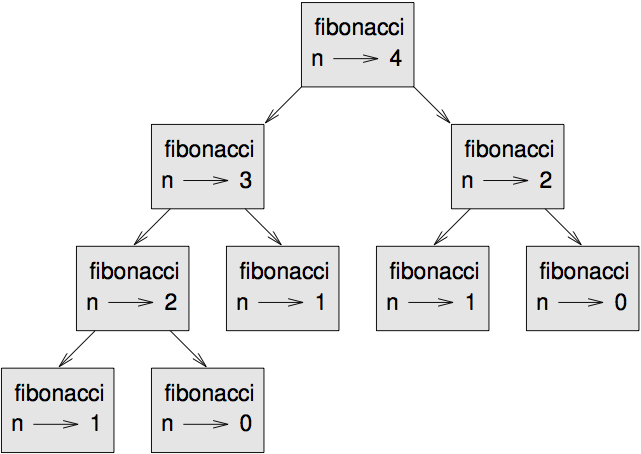
\includegraphics[scale=0.7]{figs/fibonacci.pdf}}
\caption{Call graph.}
\label{fig.fibonacci}
\end{figure}

A call graph shows a set of function frames, with lines connecting each
frame to the frames of the functions it calls.  At the top of the
graph, {\tt fibonacci} with {\tt n=4} calls {\tt fibonacci} with {\tt
n=3} and {\tt n=2}.  In turn, {\tt fibonacci} with {\tt n=3} calls
{\tt fibonacci} with {\tt n=2} and {\tt n=1}.  And so on.
\index{function frame}
\index{frame}
\index{call graph}

Count how many times {\tt fibonacci(0)} and {\tt fibonacci(1)} are
called.  This is an inefficient solution to the problem, and it gets
worse as the argument gets bigger.
\index{memo}

One solution is to keep track of values that have already been
computed by storing them in a dictionary.  A previously computed value
that is stored for later use is called a {\bf memo}.  Here is a
``memoized'' version of {\tt fibonacci}:

\begin{verbatim}
known = {0:0, 1:1}

def fibonacci(n):
    if n in known:
        return known[n]

    res = fibonacci(n-1) + fibonacci(n-2)
    known[n] = res
    return res
\end{verbatim}
%
{\tt known} is a dictionary that keeps track of the Fibonacci
numbers we already know.  It starts with
two items: 0 maps to 0 and 1 maps to 1.

Whenever {\tt fibonacci} is called, it checks {\tt known}.
If the result is already there, it can return
immediately.  Otherwise it has to 
compute the new value, add it to the dictionary, and return it.

\begin{exercise}

Run this version of {\tt fibonacci} and the original with
a range of parameters and compare their run times.

\end{exercise}

\begin{exercise}

Memoize the Ackermann function from Exercise~\ref{ackermann} and see if
memoization makes it possible to evaluate the function with bigger
arguments.  Hint: no.
Solution: \url{http://thinkpython.com/code/ackermann_memo.py}.
\index{Ackermann function}
\index{function!ack}

\end{exercise}


\section{Global variables}
\index{global variable}
\index{variable!global}

In the previous example, {\tt known} is created outside the function,
so it belongs to the special frame called \verb"__main__".
Variables in \verb"__main__" are sometimes called {\bf global}
because they can be accessed from any function.  Unlike local
variables, which disappear when their function ends, global variables
persist from one function call to the next.
\index{flag}

It is common to use global variables for {\bf flags}; that is, 
boolean variables that indicate (``flag'') whether a condition
is true.  For example, some programs use
a flag named {\tt verbose} to control the level of detail in the
output:

\begin{verbatim}
verbose = True

def example1():
    if verbose:
        print 'Running example1'
\end{verbatim}
%
If you try to reassign a global variable, you might be surprised.
The following example is supposed to keep track of whether the
function has been called:
\index{multiple assignment}
\index{assignment!multiple}

\begin{verbatim}
been_called = False

def example2():
    been_called = True         # WRONG
\end{verbatim}
%
But if you run it you will see that the value of \verb"been_called"
doesn't change.  The problem is that {\tt example2} creates a new local
variable named \verb"been_called".  The local variable goes away when
the function ends, and has no effect on the global variable.
\index{global statement}
\index{statement!global}
\index{declaration}

To reassign a global variable inside a function you have to
{\bf declare} the global variable before you use it:

\begin{verbatim}
been_called = False

def example2():
    global been_called 
    been_called = True
\end{verbatim}
%
The {\tt global} statement tells the interpreter
something like, ``In this function, when I say \verb"been_called", I
mean the global variable; don't create a local one.''
\index{update!global variable}
\index{global variable!update}

Here's an example that tries to update a global variable:

\begin{verbatim}
count = 0

def example3():
    count = count + 1          # WRONG
\end{verbatim}
%
If you run it you get:
\index{UnboundLocalError}
\index{exception!UnboundLocalError}

\begin{verbatim}
UnboundLocalError: local variable 'count' referenced before assignment
\end{verbatim}
%
Python assumes that {\tt count} is local, which means
that you are reading it before writing it.  The solution, again,
is to declare {\tt count} global.
\index{counter}

\begin{verbatim}
def example3():
    global count
    count += 1
\end{verbatim}
%
If the global value is mutable, you can modify it without
declaring it:
\index{mutability}

\begin{verbatim}
known = {0:0, 1:1}

def example4():
    known[2] = 1
\end{verbatim}
%
So you can add, remove and replace elements of a global list or
dictionary, but if you want to reassign the variable, you
have to declare it:

\begin{verbatim}
def example5():
    global known
    known = dict()
\end{verbatim}
%

\section{Long integers}
\index{long integer}
\index{integer!long}
\index{type!long}

If you compute {\tt fibonacci(50)}, you get:

\begin{verbatim}
>>> fibonacci(50)
12586269025L
\end{verbatim}
%
The {\tt L} at the end indicates that the result is a long
integer, or type {\tt long}.  In Python 3, {\tt long} is gone; all integers,
even really big ones, are type {\tt int}.
\index{Python 3}

Values with type {\tt int} have a limited range;
long integers can be arbitrarily big, but as they get bigger
they consume more space and time.

The mathematical operators work on long integers, and the functions
in the {\tt math} module, too, so in general any code that
works with {\tt int} will also work with {\tt long}.

Any time the result of a computation is too big to be represented with
an integer, Python converts the result as a long integer:

\begin{verbatim}
>>> 1000 * 1000
1000000
>>> 100000 * 100000
10000000000L
\end{verbatim}
%
In the first case the result has type {\tt int}; in the
second case it is {\tt long}.

\begin{exercise}
\index{encryption}
\index{RSA algorithm}
\index{algorithm!RSA}

Exponentiation of large integers is the basis of common
algorithms for public-key encryption.  Read the Wikipedia
page on the RSA algorithm (\url{http://en.wikipedia.org/wiki/RSA_(algorithm)})
and write functions to encode and decode messages.

% TODO: solution for this one!

\end{exercise}


\section{Debugging}
\index{debugging}

As you work with bigger datasets it can become unwieldy to
debug by printing and checking data by hand.  Here are some
suggestions for debugging large datasets:

\begin{description}

\item[Scale down the input:] If possible, reduce the size of the
dataset.  For example if the program reads a text file, start with
just the first 10 lines, or with the smallest example you can find.
You can either edit the files themselves, or (better) modify the
program so it reads only the first {\tt n} lines.

If there is an error, you can reduce {\tt n} to the smallest
value that manifests the error, and then increase it gradually
as you find and correct errors.

\item[Check summaries and types:] Instead of printing and checking the
entire dataset, consider printing summaries of the data: for example,
the number of items in a dictionary or the total of a list of numbers.

A common cause of runtime errors is a value that is not the right
type.  For debugging this kind of error, it is often enough to print
the type of a value.

\item[Write self-checks:]  Sometimes you can write code to check
for errors automatically.  For example, if you are computing the
average of a list of numbers, you could check that the result is
not greater than the largest element in the list or less than
the smallest.  This is called a ``sanity check'' because it detects
results that are ``insane.''
\index{sanity check}
\index{consistency check}

Another kind of check compares the results of two different
computations to see if they are consistent.  This is called a
``consistency check.''

\item[Pretty print the output:] Formatting debugging output
can make it easier to spot an error.  We saw an example in
Section~\ref{factdebug}.  The {\tt pprint} module provides
a {\tt pprint} function that displays built-in types in
a more human-readable format.
\index{pretty print}
\index{pprint module}
\index{module!pprint}

\end{description}

Again, time you spend building scaffolding can reduce
the time you spend debugging.
\index{scaffolding}

\section{Glossary}

\begin{description}

\item[dictionary:] A mapping from a set of keys to their
corresponding values.
\index{dictionary}

\item[key-value pair:] The representation of the mapping from
a key to a value.
\index{key-value pair}

\item[item:] Another name for a key-value pair.
\index{item!dictionary}

\item[key:] An object that appears in a dictionary as the
first part of a key-value pair.
\index{key}

\item[value:] An object that appears in a dictionary as the
second part of a key-value pair.  This is more specific than
our previous use of the word ``value.''
\index{value}

\item[implementation:] A way of performing a computation.
\index{implementation}

\item[hashtable:] The algorithm used to implement Python
dictionaries.
\index{hashtable}

\item[hash function:] A function used by a hashtable to compute the
location for a key.
\index{hash function}

\item[hashable:] A type that has a hash function.  Immutable
types like integers,
floats and strings are hashable; mutable types like lists and
dictionaries are not.
\index{hashable}

\item[lookup:] A dictionary operation that takes a key and finds
the corresponding value.
\index{lookup}

\item[reverse lookup:] A dictionary operation that takes a value and finds
one or more keys that map to it.
\index{reverse lookup, dictionary}

\item[singleton:] A list (or other sequence) with a single element.
\index{singleton}

\item[call graph:] A diagram that shows every frame created during
the execution of a program, with an arrow from each caller to
each callee. 
\index{call graph}
\index{diagram!call graph}

\item[histogram:] A set of counters.
\index{histogram}

\item[memo:] A computed value stored to avoid unnecessary future 
computation.
\index{memo}

\item[global variable:]  A variable defined outside a function.  Global
variables can be accessed from any function.
\index{global variable}

\item[flag:] A boolean variable used to indicate whether a condition
is true.
\index{flag}

\item[declaration:] A statement like {\tt global} that tells the
interpreter something about a variable.
\index{declaration}

\end{description}

\section{Exercises}

\begin{exercise}
\index{duplicate}

If you did Exercise~\ref{duplicate}, you already have
a function named \verb"has_duplicates" that takes a list
as a parameter and returns {\tt True} if there is any object
that appears more than once in the list.

Use a dictionary to write a faster, simpler version of
\verb"has_duplicates". 
Solution: \url{http://thinkpython.com/code/has_duplicates.py}.

\end{exercise}


\begin{exercise}
\label{exrotatepairs}
\index{letter rotation}
\index{rotation!letters}

Two words are ``rotate pairs'' if you can rotate one of them
and get the other (see \verb"rotate_word" in Exercise~\ref{exrotate}).

Write a program that reads a wordlist and finds all the rotate
pairs.  Solution: \url{http://thinkpython.com/code/rotate_pairs.py}.

\end{exercise}


\begin{exercise}
\index{Car Talk}
\index{Puzzler}

Here's another Puzzler from {\em Car
Talk} (\url{http://www.cartalk.com/content/puzzlers}):

\begin{quote}
This was sent in by a fellow named Dan O'Leary. He came upon a common
one-syllable, five-letter word recently that has the following unique
property. When you remove the first letter, the remaining letters form
a homophone of the original word, that is a word that sounds exactly
the same. Replace the first letter, that is, put it back and remove
the second letter and the result is yet another homophone of the
original word. And the question is, what's the word?

Now I'm going to give you an example that doesn't work. Let's look at
the five-letter word, `wrack.' W-R-A-C-K, you know like to `wrack with
pain.' If I remove the first letter, I am left with a four-letter
word, 'R-A-C-K.' As in, `Holy cow, did you see the rack on that buck!
It must have been a nine-pointer!' It's a perfect homophone. If you
put the `w' back, and remove the `r,' instead, you're left with the
word, `wack,' which is a real word, it's just not a homophone of the
other two words.

But there is, however, at least one word that Dan and we know of,
which will yield two homophones if you remove either of the first two
letters to make two, new four-letter words. The question is, what's
the word?
\end{quote}
\index{homophone}
\index{reducible word}
\index{word, reducible}

You can use the dictionary from Exercise~\ref{wordlist2} to check
whether a string is in the word list.

To check whether two words are homophones, you can use the CMU
Pronouncing Dictionary.  You can download it from
\url{http://www.speech.cs.cmu.edu/cgi-bin/cmudict} or from
\url{http://thinkpython.com/code/c06d} and you can also download
\url{http://thinkpython.com/code/pronounce.py}, which provides a function
named \verb"read_dictionary" that reads the pronouncing dictionary and
returns a Python dictionary that maps from each word to a string that
describes its primary pronunciation.

Write a program that lists all the words that solve the Puzzler.
Solution: \url{http://thinkpython.com/code/homophone.py}.

\end{exercise}



